\documentclass[12pt]{article}
\usepackage[utf8]{inputenc}
\usepackage{amsmath}
\usepackage{times}
\usepackage{amsfonts}
\usepackage{amssymb}
\usepackage{graphicx}
\usepackage{tabularx}
\usepackage[font=small,labelfont=bf]{caption}
\usepackage[font=small]{subcaption}
\usepackage{wrapfig}
\usepackage[section]{placeins}




\begin{document}
\vspace{20mm}

{\LARGE One-dimensional traveling waves in neuronal columns - supplemental information}

\ \\
{\bf \large Vincent Baker, vjb42@drexel.edu$^{\displaystyle 1}$}\\
{\bf \large Luis Cruz, ccruz@drexel.edu$^{\displaystyle 1}$}\\
{$^{\displaystyle 1}$Drexel University, Department of Physics.}\\

\pagebreak

\subsection*{Wave detection and labeling}
To automatically identify waves we perform a spatial clustering operation to this data to identify spatiotemporal regions identified by high firing density. 
The clustering operation produces an output cluster for any group of more than $3$ spike events that fall within a $20ms$ time window from neurons that are no more than $3$ layers apart.
Each cluster $C(t,z)$ has a time $t$ and position $z$.
This clustering removes random background firing activity. 
The waves are identified using a plane sweep algorithm that proceeds along the dimension of simulation time and applies wave labels to clusters such that all clusters with the same label are part of the same wave.
When a new cluster $C(t,z)$ is encountered, the algorithm associates $C(t,z)$ with any existing wave if the existing wave has a cluster $C(t_c,z_c)$ within $40 ms$ and $6$ units of the new cluster.
If there is no such adjacent cluster a new wave is created using $C(t,z)$ as the first cluster.
\begin{figure}[!htb]
 \caption{The clustering and wave labeling process. Spike raster plot (left), filtered clusters (middle) and labeled waves (right, each color is a unique wave) are shown for SCE with different values of $K$. }
 \label{fig:detector_test}
 \centering
   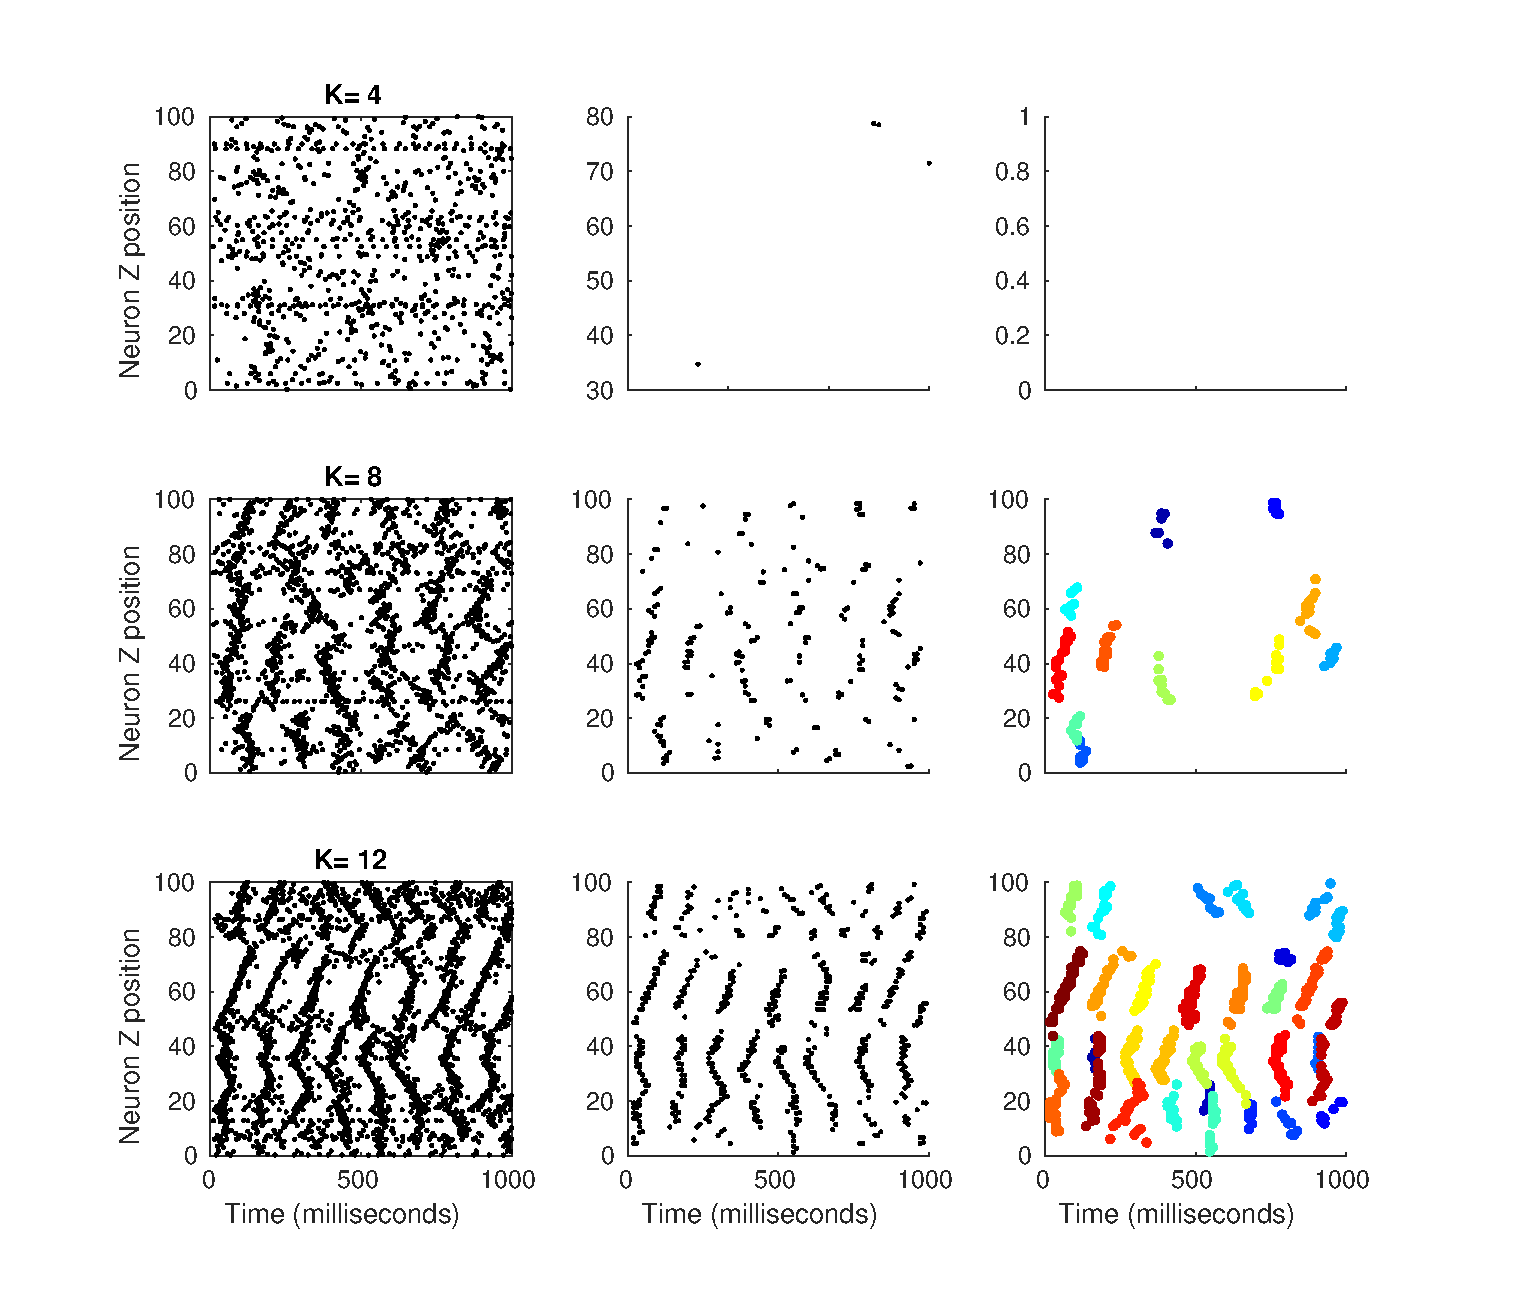
\includegraphics[width=\textwidth]{fig/DetectorTest}
\end{figure}
\FloatBarrier
 
\subsection*{Example FIE and FFE plots}
\begin{figure}[!htb]
 \caption{FIE and FFE for nine example columns. } 
 \begin{tabular}{ccc}
     \includegraphics[width=0.3\textwidth]{fig/ccf/ccf1} & \includegraphics[width=0.3\textwidth]{fig/ccf/ccf2} & \includegraphics[width=0.3\textwidth]{fig/ccf/ccf3} \\
     \includegraphics[width=0.3\textwidth]{fig/ccf/ccf4} & \includegraphics[width=0.3\textwidth]{fig/ccf/ccf5} & \includegraphics[width=0.3\textwidth]{fig/ccf/ccf6} \\
     \includegraphics[width=0.3\textwidth]{fig/ccf/ccf7} & \includegraphics[width=0.3\textwidth]{fig/ccf/ccf8} & \includegraphics[width=0.3\textwidth]{fig/ccf/ccf9} 
 \end{tabular}
\end{figure}

\FloatBarrier
 
\end{document}
